\chapter{Performance results} % Main chapter title

\label{Chapter4} 

\section{Largest contentful paint}

\begin{figure}[h!]
	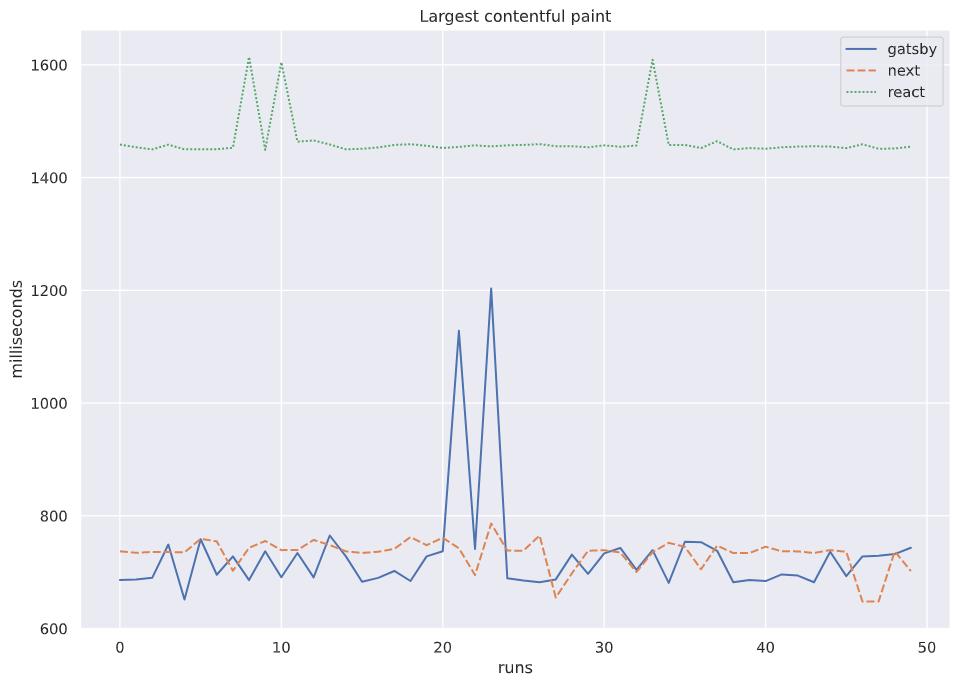
\includegraphics[scale=0.4]{largest_contentful_paint}
	\caption{Results of performance benchmark for largest contentful paint}
	\label{fig:largest_contentful_paint}
\end{figure}

In the figure, it is clear that LCP for a traditional React application is far greater than that of static site generators.

This makes sense: a traditional React application will perform many computational steps during runtime to render the DOM.
Static site generators will perform these computations during the build step.

\section{Total blocking time}


\begin{figure}[h!]
	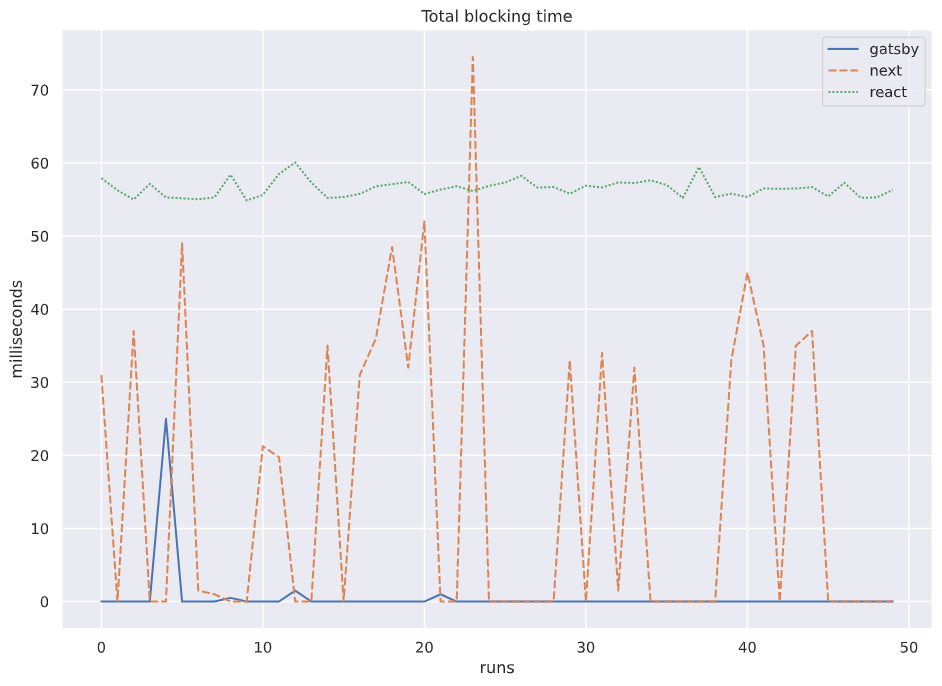
\includegraphics[scale=0.4]{total_blocking_time}
	\caption{Results of performance benchmark for total blocking time}
	\label{fig:total_blocking_time}
\end{figure}

Similar results from the previous figure can be observed. 
The traditional React application scores much less favorably than the static site generators.
Interestingly, the results for Next seem to spike a lot.

\section{Bundle size}

To measure the size of the resulting files after a production build was measured with the Unix command 

\begin{verbatim}
	du -c <directory>
\end{verbatim}

\begin{table}[h!]
	\begin{center}
		\begin{tabular}{||c c||} 
			\hline
			Site   & Col2 \\ [0.5ex] 
			\hline\hline
			Gatsby & 3072 \\ 
			\hline
			Next   & 7012 \\
			\hline
			React  & 568  \\[1ex] 
			\hline
		\end{tabular}
		\caption{Total file size of production builds, in kilobytes }
	\end{center}
\end{table}

The traditional React application has the smallest bundle here. 
This makes sense, the static generators Next and Gatsby will bundle assets while the traditional React app will fetch these during runtime.

While these results are interesting to see, it should not be a definite factor when deciding which technology to use.
The PoCs created for this paper are very small, a real application would have orders of magnitude more lines of code.
Minification really shines with larger codebases. 